%!TEX program = xelatex
\documentclass[aspectratio=169]{ctexbeamer}
\usepackage[list=true]{subcaption}
% \usepackage{physics}  
                        %%% 宽高比说明 %%%%
%% ctexbeamer宏包支持各种宽高比,但本模板只适配了4:3(默认)和16:9的宽高比背景。
%% 添加选项aspectratio=169或aspectratio=43可以更改宽高比,默认是4:3
\usepackage[bluetheme]{ustcbeamer}
\input{ustctheme.tex}
                        %%% ustcbeamer说明 %%%%
%% 宏包使用了TikZ代码形式的背景文件(在子文件夹theme中),默认选项"bluetheme",是科大校徽的蓝色;此外ustcbeamer还内置了红色和黑色主题"redtheme","blacktheme"。

                        %%% 自定义你的主题颜色 %%%
%% 一旦使用了下述命令就会覆盖ustcbeamer的内置颜色选项,你可以设置自己喜欢的RGB色值:
% \definecolor{themecolor}{RGB}{0,150,0} % 这是绿色主题
% \definecolor{themecolor}{RGB}{0,150,150} % 青色主题,也蛮好看的

%% 注意小写rgb和大写RGB表示的色值相差255倍,即RGB{255,255,255}=rgb{1,1,1};
% \definecolor{themecolor}{rgb}{0,0.5,0.3} % 深绿色主题

%% 建议自定义的主题颜色选择偏深色
%%%%%%%%%%%%%%%%%%%%%%%%%%%%%%%%%%%%%%%%%%%%%%%%%%%%%%%%%%%%%%%%%%%%%%


\title[加倍空间下的核心集]{
  毕业论文答辩————加倍空间下的核心集
}
\author[沈俊杰]{答辩人:沈俊杰}
\institute[USTC]{
中国科学技术大学,计算机科学与技术系
}
\date{\today}
\begin{document}
%\section<⟨mode specification⟩>[⟨short section name⟩]{⟨section name⟩}
%小于等于六个标题为恰当的标题

%--------------------
%标题页
%--------------------
\maketitleframe
%--------------------
%目录页
%--------------------
%beamer 101
\begin{frame}%
	\frametitle{大纲}%
	\tableofcontents[hideallsubsections]%仅显示节
	%\tableofcontents%显示所节和子节
\end{frame}%
%--------------------
%节目录页
%--------------------
\AtBeginSection[]{
\setbeamertemplate{footline}[footlineoff]%取消页脚
  \begin{frame}%
    \frametitle{大纲}
	%\tableofcontents[currentsection,subsectionstyle=show/hide/hide]%高亮当前节,不显示子节
    \tableofcontents[currentsection,subsectionstyle=show/show/hide]%show,shaded,hide
  \end{frame}
\setbeamertemplate{footline}[footlineon]%添加页脚
}
%--------------------
%子节目录页 maybe delete this part
%--------------------
\AtBeginSubsection[]{
\setbeamertemplate{footline}[footlineoff]%取消页脚
  \begin{frame}%
    \frametitle{大纲}
	%\tableofcontents[currentsection,subsectionstyle=show/hide/hide]%高亮当前节,不显示子节
    \tableofcontents[currentsection,subsectionstyle=show/shaded/hide]%show,shaded,hide
  \end{frame}
\setbeamertemplate{footline}[footlineon]%添加页脚
}

\section{论文简介}
\begin{frame}
  \frametitle{论文简介}
  本论文使用了一种动态更新的算法框架,为满足特定条件的一类CnB机器学习问题构建鲁棒核心集(coreset),并
  在理论上证明了该核心集大小的复杂度下界与参数空间$\mathcal{P}$的加倍维度有关,在现实数据集上进行鲁棒性相关的实验测试。  
\end{frame}


\section{研究背景}
\begin{frame}
  \frametitle{研究背景}
在处理一个机器学习任务时,此时我们希望构建一个小的数据集,例如核心集,用以表征原始数据集的一些特性。
核心集是一种有良好理论保证的数据压缩方法,一个$\varepsilon$-coreset$C$指:
\begin{equation*}
  \forall \theta \in \mathcal{P},(1-\varepsilon)f(\theta,X)\leq f(\theta,C)    \leq(1+\varepsilon)f(\theta,X)
\end{equation*}
其中$f$和$\theta$是机器学习问题中的损失函数和参数,$\mathcal{P}$是参数空间,$X$是原始数据集。

在大数据时代,随着数据量的增大,我们对核心集的相关算法有了更多的要求,例如:
\begin{itemize}
  \item 核心集的大小复杂度
  \item 核心集的动态维护
  \item 核心集的鲁棒性
\end{itemize}
\end{frame}

\begin{frame}
  \frametitle{鲁棒性}
  鲁棒性是指核心集在面对数据集中的异常点时,仍然能够保持较好的质量。

  为什么需要鲁棒性?Sampling-based方法在面对异常点时,可能会导致核心集的质量下降。
  \pause
  
  一个$(\beta,\varepsilon)$-coreset$C$指:
  \begin{equation*}
    \forall \theta \in \mathcal{P},(1-\varepsilon)f_{(1+\beta)z}(\theta,X)\leq f_z(\theta,C)    \leq(1+\varepsilon)f_{(1-\beta)z}(\theta,X)
  \end{equation*}
\end{frame}


\section{模型框架}
\subsection{基础算法}
\begin{frame}
  \frametitle{基础算法}
  CnB问题:$f(\theta,x)$关于$\theta$是Lipchitz连续的,且参数$\theta$被限定在一个有界的空间内,不妨为$\mathbb{B}(\tilde{\theta},\ell)$,求$\min_\theta \sum_if(\theta,x_i)$
  
  \textbf{算法框架(简):} 对每个点x,利用$f(\theta,x_{\tilde{z}})$的值将其分为两类:$X_{si}$和$X_{so}$,即可疑的正常点和异常点。
  对$X_{si}$中的点,我们运行一个黑盒的已有核心集算法;对$X_{so}$中的点,我们均匀采样,合并两部分,作为输出的核心集。
\end{frame}

\subsection{动态情况}
\begin{frame}
  \frametitle{动态情况}
  \begin{figure}
    \centering
    \subcaptionbox[Short Subcaption]{%
        Merge-and-Reduce(无离群点时)%
        \label{subfig:sublabel1}%
    }
    [%
        0.45\textwidth % width of caption
    ]%
    {%
        \includegraphics[width=0.45\textwidth]%
        {./figures/merge-and-reduce.pdf}%
    }%
    \hfill
    \subcaptionbox[Short Subcaption]{%
        Merge-and-Reduce(有离群点时)%
        \label{subfig:sublabel2}%
    }
    [%
        0.45\textwidth % width of caption
    ]%
    {%
        \includegraphics[width=0.45\textwidth]%
        {./figures/merge-and-reduce-outliers.pdf}%
    }%
    \caption[Short Caption]{动态情况下的核心集框架}
    \label{fig:dyn}
  \end{figure}
  动态情况指核心集算法需要在数据流中动态地维护核心集,以适应数据的变化。

\end{frame}


\section{实验结果}
\begin{frame}
  \frametitle{衡量指标}
  在本实验中,我们使用两种损失偏差,即考虑离群点和不考虑离群点的损失偏差,分别记为$\mathbf{LR}_z$和
$\mathbf{LR}$,下标z表示核心集构建过程(以及kmeans算法)中选择的离群点的数量(权重和)。
\begin{equation*}
    \mathbf{LR} = \max\left\{\frac{f(\theta^*_C,C)}{f(\theta^*_X,X)},\frac{f(\theta^*_X,X)}{f(\theta^*_C,C)}\right\},\quad
    \mathbf{LR}_z = \max\left\{\frac{f_z(\theta^*_C,C)}{f_z(\theta^*_X,X)},\frac{f_z(\theta^*_X,X)}{f_z(\theta^*_C,C)}\right\}
\end{equation*}
其中$\theta^*_{X(C)}$是算法在$X(C)$上使用k-means算法得到的解,核心集大小和加速比分别记为$|C|$和$\mathbf{SR}$。
本实验中有一对重要参数(noise\_ratio,outliers\_ratio)。noise\_ratio表示我们在数据集中额外生成噪声的比例,
outlier\_ratio表示我们在构建核心集和运行kmeans算法时使用的参数,和分析中的离群点数量z直接相关。
实验表明,对于不同的参数对,评价指标$\mathbf{LR}_z$相较$\mathbf{LR}$而言有较大的波动,这说明该评价指标一定程度衡量了鲁棒性,也意味着我们需要针对数据集和算法选择更合适的参数。
下图展示了在MNIST数据集上不同参数的的实验结果。
\end{frame}

\begin{frame}{实验结果}

\begin{figure}
  
  \centering
    \begin{minipage}{0.8\linewidth}
        \centering
        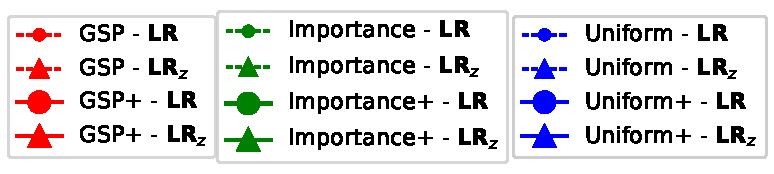
\includegraphics[width=0.5\linewidth]{./figures/legend.pdf}
        \subcaption{图(b)、(d)的图例}
    \end{minipage}
    \\
    \begin{minipage}{0.49\linewidth}
        \centering
        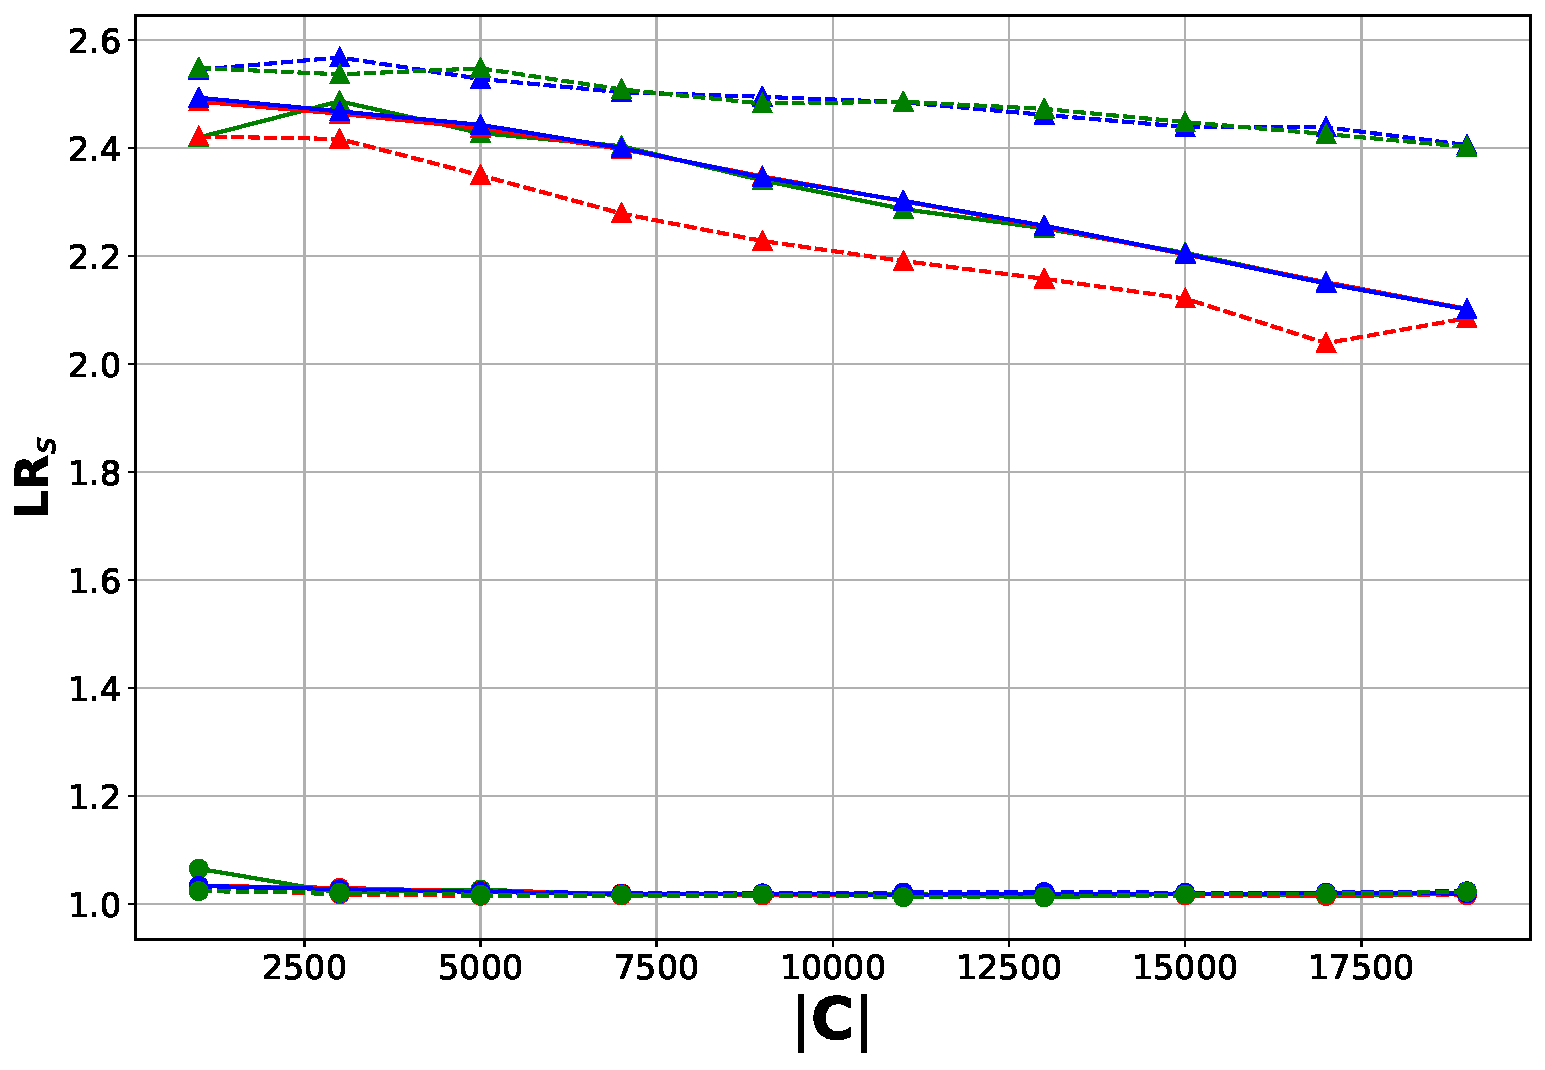
\includegraphics[width=0.85\linewidth]{./figures/loss_ratio(0.05,0.2) - MNIST.pdf}
        \subcaption{(0.05,0.2)-MNIST $\mathbf{LR},\mathbf{LR}_z$}
    \end{minipage}
    \hfill
    \begin{minipage}{0.49\linewidth}
        \centering
        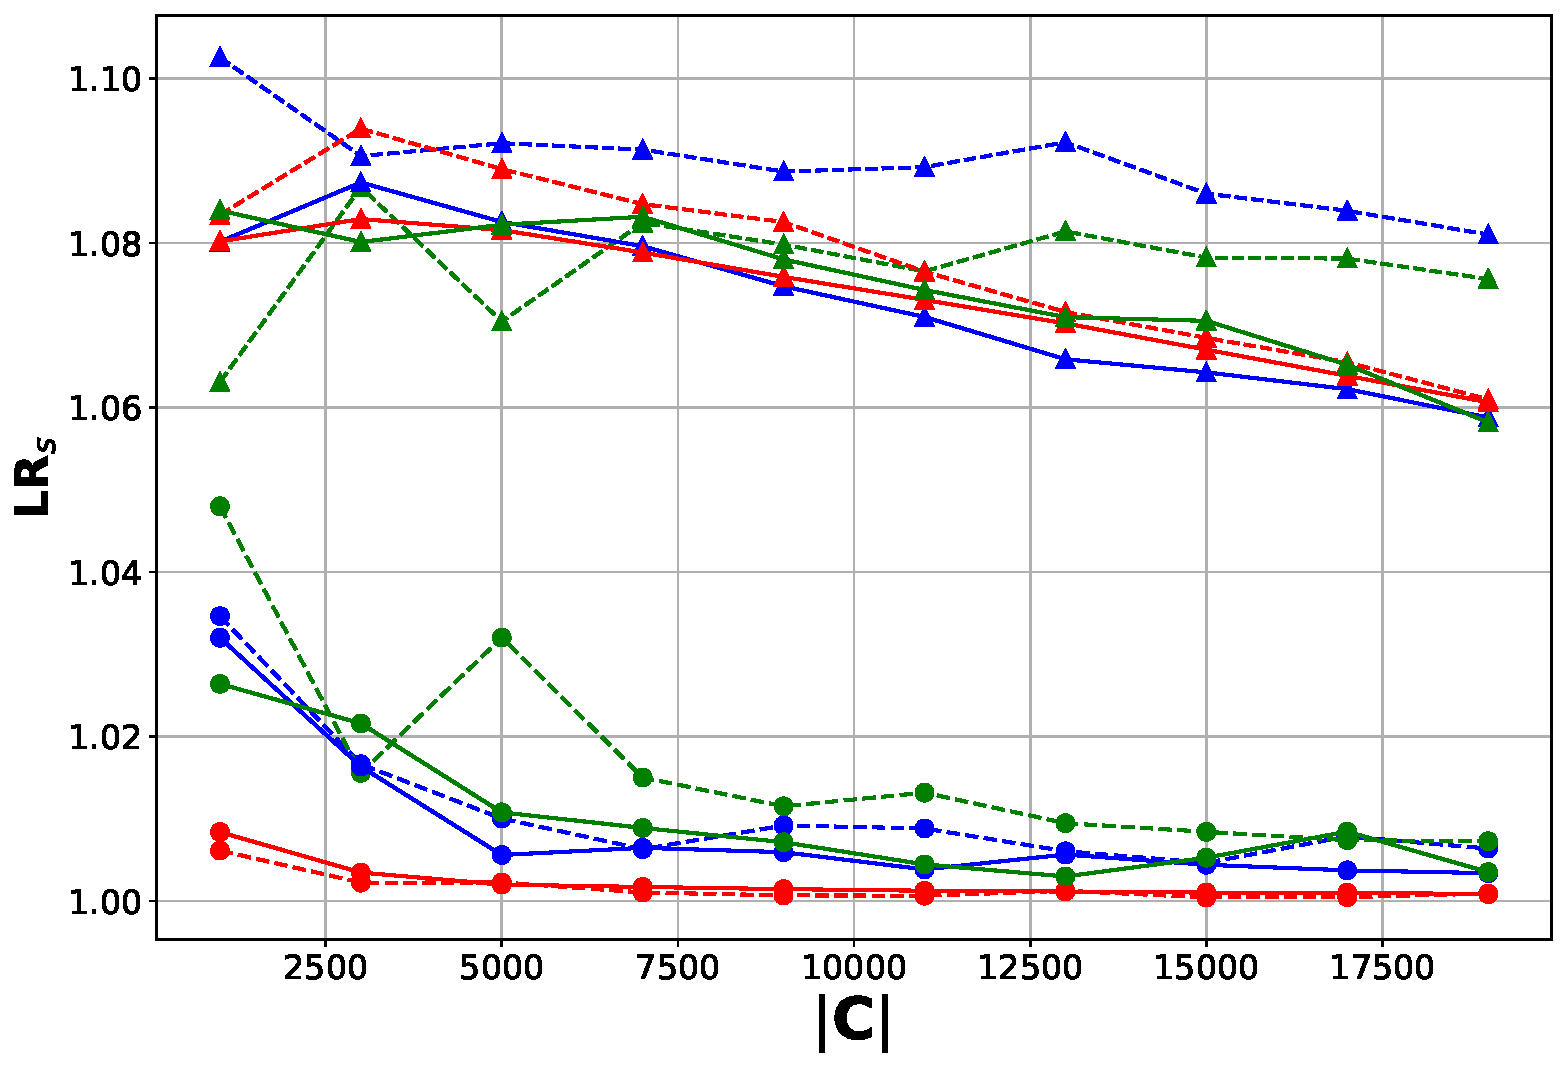
\includegraphics[width=0.85\linewidth]{./figures/loss_ratio(0.2,0.05) - MNIST.pdf}
        \subcaption{(0.2,0.05)-MNIST $\mathbf{LR},\mathbf{LR}_z$}
    \end{minipage}
    %\caption{两种参数下MNIST数据集上的表现}
    \label{fig:mnist_combined}
\end{figure}
\end{frame}


\section{理论证明}

\begin{frame}
  \frametitle{研究方法}
  \begin{block}{方法一}
    \begin{itemize}
      \item abc
      \item def
    \end{itemize}
  \end{block}
  \pause
  \begin{block}{方法二}
    \begin{itemize}
      \item abc
      \item def
    \end{itemize}
  \end{block}
\end{frame}


\section{总结展望}

\begin{frame}
  \frametitle{总结展望}
  \begin{columns}
    \begin{column}{0.50\textwidth}
      \begin{figure}
        \includegraphics[width=0.8\textwidth]{figures/ustc_logo.pdf}
        \caption{标题}
      \end{figure}
    \end{column}
    \begin{column}{0.50\textwidth}
      \begin{block}{结论}
        \begin{itemize}
          \item 结论 1
          \item 结论 2
          \item 结论 3
        \end{itemize}
      \end{block}
    \end{column}
  \end{columns}
\end{frame}

\begin{frame}
  \frametitle{致谢}
  \centerline{\Large 谢谢!}
\end{frame}

\end{document}
